\addchap{Anhang}
\label{chap:anhang}

\section{Section}

\subsection{Subsection 1}
\subsubsection{Subsubsection 1}
\subsubsection{Subsubsection 2}

\subsection{Subsection 2}
\subsubsection{Subsubsection 1}
\subsubsection{Subsubsection 2}

\section{Quelltexte}
\label{sec:quelltexte}


\begin{code}
  \lstinputlisting[language=tex]{sourcecode/LICENSE}
  \caption{MIT Lizenz}
  \label{lst:mitlizenz}
\end{code}


\section{Algorithmen}

Algorithmus \ref{alg:erstroutenplanung-anhang} zeigt auf, wie eine Generierung einer mäanderförmigen Erstroutenplanung erfolgt \citep[S.~42]{Bachelorthesis.2016}.

\begin{algorithm}
  \caption{Mäanderförmige Erstroutenplanung}
  \label{alg:erstroutenplanung-anhang}
  \begin{algorithmic}[1]
    \Require{
      \parbox[t]{.89\linewidth}{
        Flugzellenmatrizen $X^{m\times n}\;,Y^{m\times n}$
      }
    }
    \Ensure{Flugroute $F=(f_1,\; f_2,\; \dots,\; f_n)$}
    \Procedure{GetMeanderFlightRoute}{$X, Y$}
    \State $F=()$
    \State $a=1$

    \For{$i = 1:m$}
      \If{$i \bmod 2 \neq 0$}
        \For{$j = 1:n$}
          \State $f_a = (x_{ij}, y_{ij})$
          \State $a=a+1$
        \EndFor
      \Else
        \For{$j = n:1$}
          \State $f_a = (x_{ij}, y_{ij})$
          \State $a=a+1$
        \EndFor
      \EndIf
    \EndFor

    \State \Return $F$

    \EndProcedure
  \end{algorithmic}
\end{algorithm}

\section{Bilder}

Bilder aus dem Anhang werden nicht im Abbildungsverzeichnis aufgeführt, daher ist dort auch kein Link zu \ref{fig:zeitreihe-komponenten4}.

\begin{figure}[h]
  \centering
  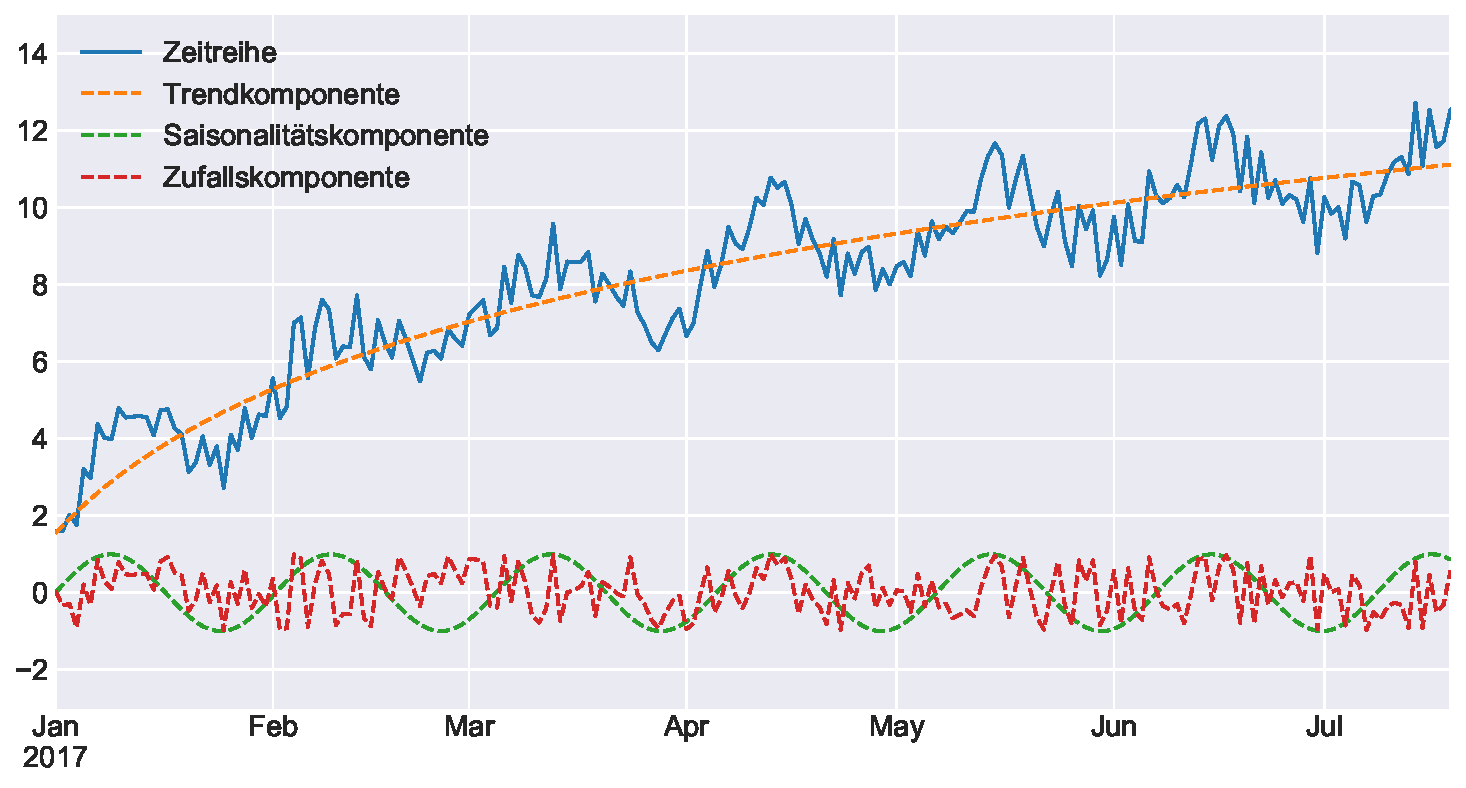
\includegraphics[width=\textwidth]{bilder/02-hauptteil/zeitreihe-komponenten.pdf}
  \caption[Aufteilung einer Zeitreihe in mehrere Komponenten]{Aufteilung einer Zeitreihe in mehrere Komponenten. Bild entnommen aus \citet{Masterthesis.2017}.}
  \label{fig:zeitreihe-komponenten4}
\end{figure}

\section{Tabelle}
\ref{tbl:gg-hoofed-stock} ist eine Tabelle im Anhang.
\begin{table}[ht]
  \centering
  % Tabular example from LaTeX manual, p.205
  \begin{tabular}{|r||r@{--}l|p{38mm}|}
    \hline
    \mc{4}{|c|}{GG\&A Hoofed Stock}\\ \hline \hline
     & \mc{2}{c|}{Price} & \\ \cline{2-3}
    \mc{1}{|c||}{Year} & \mc{1}{r@{\,\vline\,}}{low} & high & \mc{1}{c|}{Comments} \\ \hline
    1971 & 97 & 245 & Bad year for farmers in the west. \\ \hline
      72 & 245 & 245 & Light trading due to a heavy winter. \\ \hline
      73 & 245 & 2001 & No gnus was very good gnus this year. \\ \hline
  \end{tabular}
  \caption[GG\&A Hoofed Stock]{GG\&A Hoofed Stock. Tabelle mit Priotität der Position unmittelbar an der Stelle im Quellcode durch kennzeichnen mit \texttt{ht}. Abgeändert übernommen von \url{https://mirror.hmc.edu/ctan//info/examples/lb2/5-7-8.ltx}.}
  \label{tbl:gg-hoofed-stock}
\end{table}


\section{Inhalte des beiliegenden Datenträgers}
\label{sec:quelltexte}
Kein Datenträger vorhanden.
